\documentclass{article}
\usepackage{geometry}
\usepackage{fancyhdr}
%\usepackage{amsmath,amsthm,amssymb}
\usepackage{graphicx}
\usepackage{hyperref}
\usepackage{ntheorem}
\newtheorem{hyp}{Hypothesis}

\title{Results Section}
\author{Me}
\date{22-December-2015}
\begin{document}
\maketitle
\graphicspath{ {../Plots/} }

\section{Arterial}
\begin{table}[ht]
\centering
\begin{tabular}{rrr}
  \hline
 & Trained & Untrained \\ 
  \hline
1 & 144.00 & 480.00 \\ 
  2 & 175.00 & 480.00 \\ 
  3 & 287.00 & 480.00 \\ 
  4 & 207.00 & 480.00 \\ 
   \hline
\end{tabular}
\end{table}

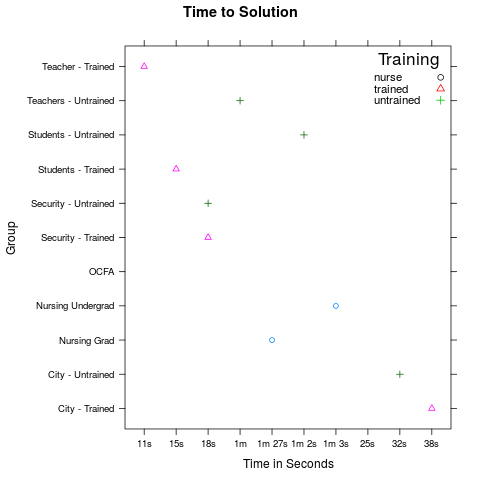
\includegraphics[width = 10cm]{Arterial_Time.png}

\section{Airway}
\begin{table}[ht]
\centering
\begin{tabular}{rrr}
  \hline
 & airwayTrained & airwayUntrained \\ 
  \hline
1 & 11.00 & 480.00 \\ 
  2 & 38.00 & 480.00 \\ 
  3 & 18.00 & 160.00 \\ 
  4 & 15.00 & 480.00 \\ 
   \hline
\end{tabular}
\end{table}

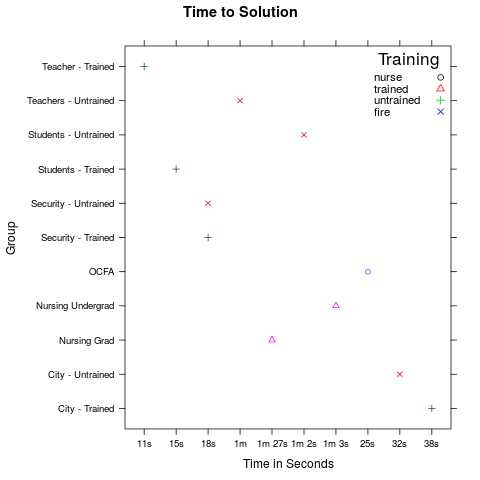
\includegraphics[width = 10cm]{Airway_Time.png}

\end{document}

